\documentclass{../mathhomework}
\usepackage{enumitem}
\usepackage{graphicx}
\usepackage{float}

\newcommand{\Let}{\textit{let }}
\newcommand{\Span}[1]{\textit{Span}\{#1\}}
\newcommand{\Powerset}[1]{\mathcal{P}(#1)}
\newcommand{\By}[1]{\text{(by #1)}}
\newcommand{\circnum}[1]{\text{\textcircled{#1}}}

\newenvironment{Mat}{\begin{bmatrix}}{\end{bmatrix}}

% Assigment Info
\coursetitle{Linear Algebra}
\courseinstructor{Professor MacArthur}

\student{Carson Storm}

\assignmenttitle{Homework \#2}
\assignmentduedate{September 4, 2019}

% Section 1.6 #4, 7, 11, 13
% Section 1.7 #1, 3, 5, 7, 11, 13, 15, 17, 19, 21, 23, 25
% Section 1.8 #1, 2, 3, 5, 7, 9, 11, 13, 16, 30, 33

\begin{document}
\maketitle

\pagebreak

\begin{problem}[1.6\#4]
    Suppose an economy has four sectors, Agriculture (A), Energy (E), Manufacturing (M), and Transportation (T). 
    Sector A sells 10\% of its output to E and 25\% to M and reatins the rese. Sectore E sells 30\% of its output
    to A, 35\% to M, and 25\% to T and reatins the rest. Sector M sells 30\% of its output to A, 15\% to E, and 40\%
    to T and reatins the rest. Sector T sells 20\% of its output to A, 10\% to E, and 30\% to M and retains the rest.
    \begin{enumerate}[label=\alph*.]
        \item Construct the exchange table for this economy.
        \item $[M]$ Find a set of equilibrium prices for the economy.
    \end{enumerate}
\end{problem}

\begin{problem}[1.6\#7]
    Alka-Seltzer contains sodium bicarbonate ($NaHCO_3$) and citric acid ($H_3C_6H_5O_7$). When a tablet is dissolved
    in water, the following reaction produces sodium citrate, water, and carbon dioxide (gas):
    \begin{equation*}
        NaHCO_3 + H_3C_6H_5O_7 \to Na_3C_6H_5O_7 + H_2O + CO_2
    \end{equation*}
    Balance the chemical equaion using the vector equation approach.
\end{problem}

\begin{problem}[1.6\#11]
    Find the general flow pattern of the network shown in the figure. Assuming that the flows are all nonnegative, what
    is the largest possible value for $x_3$?

    \begin{figure}[h!]
        \begin{center}
            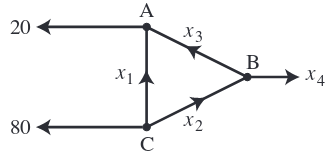
\includegraphics[width=2in]{figures/1_6_11.png}
        \end{center}
    \end{figure}
\end{problem}

\begin{problem}[1.6\#13]
    \begin{enumerate}[label=\alph*.]
        \item Find the general flow pattern in the network shown in the figure.
        \item Assuming that the flow must be in the directions indicated, find the minimum flows in the branches denoted by $x_2,x_3,x_4$ and $x_5$.
    \end{enumerate}

    \begin{figure}[h!]
        \begin{center}
            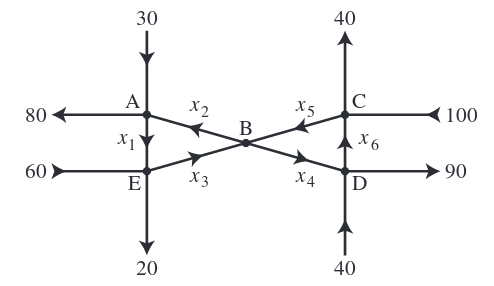
\includegraphics[width=2in]{figures/1_6_13.png}
        \end{center}
    \end{figure}
\end{problem}

\begin{problem}[1.7\#1]
    Determine if the vectors are linearly independent. Justify answer.
    
    \begin{equation*}
        \begin{Mat}
            5 \\ 0 \\ 0
        \end{Mat},
        \begin{Mat}
            7 \\ 2 \\ -6
        \end{Mat},
        \begin{Mat}
            9 \\ 4 \\ -8
        \end{Mat}
    \end{equation*}
\end{problem}

\begin{problem}[1.7\#3]
    Determine if the vectors are linearly independent. Justify answer.
    
    \begin{equation*}
        \begin{Mat}
            1 \\ -3
        \end{Mat},
        \begin{Mat}
            -3 \\ 9
        \end{Mat}
    \end{equation*}
\end{problem}

\begin{problem}[1.7\#5]
    Determine if the columns of the matrix form a linearly independent set. Justify your answer.

    \begin{equation*}
        \begin{Mat}
            0 & -8 & 5 \\
            3 & -7 & 4 \\
            -1 & 5 & -4 \\
            1 & -3 & 2
        \end{Mat}
    \end{equation*}
\end{problem}

\begin{problem}[1.7\#7]
    Determine if the columns of the matrix form a linearly independent set. Justify your answer.

    \begin{equation*}
        \begin{Mat}
            1 & 4 & -3 & 0 \\
            -2 & -7 & 5 & 1 \\
            -4 & -5 & 7 & 5
        \end{Mat}
    \end{equation*}
\end{problem}

\begin{problem}[1.7\#11]
    Find the value(s) of $h$ for which the vectors are linearly dependent. Justify your answer.

    \begin{equation*}
        \begin{Mat}
            1 \\ -1 \\ 4
        \end{Mat},
        \begin{Mat}
            3 \\ -5 \\ 7
        \end{Mat},
        \begin{Mat}
            -1 \\ 5 \\ h
        \end{Mat}
    \end{equation*}
\end{problem}

\begin{problem}[1.7\#13]
    Find the value(s) of $h$ for which the vectors are linearly dependent. Justify your answer.

    \begin{equation*}
        \begin{Mat}
            1 \\ 5 \\ -3
        \end{Mat},
        \begin{Mat}
            -2 \\ -9 \\ 6
        \end{Mat},
        \begin{Mat}
            3 \\ h \\ -9
        \end{Mat}
    \end{equation*}
\end{problem}

\begin{problem}[1.7\#15]
    Determine by inspection whether the vectors are linearly independent. Justify your answer.

    \begin{equation*}
        \begin{Mat}
            5 \\ 1
        \end{Mat},
        \begin{Mat}
            2 \\ 8
        \end{Mat},
        \begin{Mat}
            1 \\ 3
        \end{Mat},
        \begin{Mat}
            -1 \\ 7
        \end{Mat}
    \end{equation*}
\end{problem}

\begin{problem}[1.7\#17]
    Determine by inspection whether the vectors are linearly independent. Justify your answer.

    \begin{equation*}
        \begin{Mat}
            3 \\ 5 \\ -1
        \end{Mat},
        \begin{Mat}
            0 \\ 0 \\ 0
        \end{Mat},
        \begin{Mat}
            -6 \\ 5 \\ 4
        \end{Mat}
    \end{equation*}
\end{problem}

\begin{problem}[1.7\#19]
    Determine by inspection whether the vectors are linearly independent. Justify your answer.

    \begin{equation*}
        \begin{Mat}
            -8 \\ 12 \\ -4
        \end{Mat},
        \begin{Mat}
            2 \\ -3 \\ -1
        \end{Mat}
    \end{equation*}
\end{problem}

\begin{problem}[1.7\#21]
    Mark each statment True or False. Justify each answer on the basis of a careful reading of the text.
    
    \begin{enumerate}
        \item The columns of a matrix $A$ are linearly independent if the equation $A\Vect{x} = 0$ has the trivial solution
        \item If $S$ is a linearly dependent set, then each vector is a linear combination of the other vectors in $S$.
        \item The columns of any $4 \times 5$ matrix are linearly dependent.
        \item If $x$ and $y$ are linearly independent, and if $\{x,y,z\}$ is linearly dependent, then $z$ is in $\Span{x,y}$
    \end{enumerate}
\end{problem}

\begin{problem}[1.7\#23]
    Describe the possible echelon forms of $A$, a $3 \times 3$ matrix with linearly independent columns. Use the notation of Example 1 in Section 1.2
\end{problem}

\begin{problem}[1.7\#25]
    Describe the possible echelon forms of $A$, a $2 \times 2$ matrix with linearly dependent columns. Use the notation of Example 1 in Section 1.2
\end{problem}

\begin{problem}[1.8\#1]
    Let $A = \begin{Mat}
        2 & 0 \\
        0 & 2
    \end{Mat}$, and define $T: \R^2 \to R^2$ by $T(\Vect{x}) = A\Vect{x}$. Find the images under $T$ of $\Vect{u} = \begin{Mat}
        1 \\ -3
    \end{Mat}$, and $\Vect{v} = \begin{Mat}
        a \\ b
    \end{Mat}$.
\end{problem}

\begin{problem}[1.8\#2]
    Let $A = \begin{Mat}
        .5 & 0 & 0 \\
        0 & .5 & 0 \\
        0 & 0 & .5 \\
    \end{Mat}, \Vect{u} = \begin{Mat}
        1 \\ 0 \\ -4
    \end{Mat}$, and $\Vect{v} = \begin{Mat}
        a \\ b \\ c
    \end{Mat}$. Define $T: \R^3 \to R^3$ by $T(\Vect{x}) = A\Vect{x}$. Find $T(\Vect{u})$ and $T(\Vect{v})$.
\end{problem}

\begin{problem}[1.8\#3]
    Find a vector $\Vect{x}$ whose image under $T$ is $\Vect{b}$ and determine whether $x$ is unique. $T(\Vect{x}) = A\Vect{x}$.
    \begin{equation*}
        A = \begin{Mat}
            1 & 0 & -2 \\
            -2 & 1 & 6 \\
            3 & -2 & -5
        \end{Mat},
        \Vect{b} = \begin{Mat}
            1 \\ 9 \\ 3 \\ -6
        \end{Mat}
    \end{equation*}
\end{problem}

\begin{problem}[1.8\#5]
    Find a vector $\Vect{x}$ whose image under $T$ is $\Vect{b}$ and determine whether $x$ is unique. $T(\Vect{x}) = A\Vect{x}$.
    \begin{equation*}
        A = \begin{Mat}
            1 & -5 & -7 \\
            -3 & 7 & 5
        \end{Mat},
        \Vect{b} = \begin{Mat}
            -2 \\ -2
        \end{Mat}
    \end{equation*}
\end{problem}

\begin{problem}[1.8\#7]
    Let $A$ be $6 \times 5$ matrix. What must $a$ and $b$ be in order to define $T: \R^a \to \R^b$ by $T(x) = A\Vect{x}$?
\end{problem}

\begin{problem}[1.8\#9]
    Find all $x$ in $\R^4$ that are mapped into the zero vector by the transofmration $\Vect{x} \mapsto A\Vect{x}$ for the given matrix $A$.
    
    \begin{equation*}
        \begin{Mat}
            1 & -4 & 7 & -5 \\
            0 & 1 & -4 & 3 \\
            2 & -6 & 6 & -4
        \end{Mat}
    \end{equation*}
\end{problem}

\begin{problem}[1.8\#11]
    Let $\Vect{b} = \begin{Mat}
        -1 \\ 1 \\ 0
    \end{Mat}$, and let $A$ be the matrix be the matrix in Exercise 9. Is $\Vect{b}$ in the range of the linear transofmration $\Vect{x} \mapsto A\Vect{x}$? Why or why not?
\end{problem}

\begin{problem}[1.8\#13]
    Use a rectangular coordinate system to plot $\Vect{u} = \begin{Mat}
        5 \\ 2
    \end{Mat}$, $\Vect{v} = \begin{Mat}
        -2 \\ 4
    \end{Mat}$, and their images under the given transformation $T$. Describe geometrically what $T$ does to each vector $x$ in $\R^2$.

    \begin{equation*}
        T(\Vect{x}) = \begin{Mat}
            -1 & 0 \\
            0 & -1
        \end{Mat}
        \begin{Mat}
            x_1 \\ x_2
        \end{Mat}
    \end{equation*}
\end{problem}

\begin{problem}[1.8\#16]
    Use a rectangular coordinate system to plot $\Vect{u} = \begin{Mat}
        5 \\ 2
    \end{Mat}$, $\Vect{v} = \begin{Mat}
        -2 \\ 4
    \end{Mat}$, and their images under the given transformation $T$. Describe geometrically what $T$ does to each vector $x$ in $\R^2$.

    \begin{equation*}
        T(\Vect{x}) = \begin{Mat}
            0 & 1 \\
            1 & 0
        \end{Mat}
        \begin{Mat}
            x_1 \\ x_2
        \end{Mat}
    \end{equation*}
\end{problem}

\begin{problem}[1.8\#30]
    An \textit{affine transofmration} $T: \R^n \to R^m$ has the form $T(\Vect{x}) = A\Vect{x} + \Vect{b}$, with $A$ an $m \times n$ matrix and $\Vect{b}$ in $\R^m$.
    Show that $T$ is \textit{not} a linear transofmation when $\Vect{b} \neq 0$ 
\end{problem}

\begin{problem}[1.8\#33]
    Show that the transformation $T$ defined by $T(x_1,x_2) = (2x_1 - 3x_2, x_1 + 4, 5x_2)$ is not linear.
\end{problem}

\end{document}